\documentclass{szzclass}

\title{Čisté objektové paradigma — principy návrhu OO systémů.}

\begin{document}
\maketitle

\tableofcontents
\newpage

\section{Postup návrhu OO systémů}

\begin{enumerate}
      \item Identify minimal requirements
      \item Make requirements testable
      \item Identify objects and their responsibilities
      \item Implement and test classes
      \item Refactor to simplify design
      \item Iterate
\end{enumerate}

\section{Povinosti objektů}

\begin{itemize}
      \item uchovávat informace a poskytovat služby pracující s těmito informacemi
      \item \textbf{high cohesion} -- vysoká soudružnost operací a dat uvnitř třídy
      \item \textbf{low coupling} -- nízká provázanost mezi třídami
      (\textit{Každá třída by měla provádět právě jednu činnost})
      \item \textbf{high-level-of-abstraction} -- vysoká míra abstrakce.
      Na všechno mít speciální rozhraní a vždy používat rozhraní místo implementace.
\end{itemize}


\section{Symptomy degradujícího návrhu SW}

\begin{itemize}
      \item \textbf{Rigidity} -- SW není snadné jednoduše měnit nebo rozšiřovat,
      nelze přidávat ani jednoduché funkcionality.
      \item \textbf{Fragility} -- Změna jedné části SW ovlivní (rozbije) jinou
      část SW (třeba i konceptuálně odlišnou).
      \item \textbf{Immobility} -- Není možné znovu použít SW pro jiné projekty
      nebo alespoň pro části jiných projektů.
      \item \textbf{High design viscosity} -- Udržování správného návrhu je implementačně náročnější
      než to udělat proti pravidlům daného návrhu, což vede k degradaci návrhu.
      \item \textbf{High environment viscosity} -- Prostředí pro vývoj SW je pomalé a neefektivní.
      Například dlouhý \textit{compile-time}.
\end{itemize}


\section{Principy OO návrhu}

Dodržování následujících principů vede ke snížení provázanosti mezi třídami.
V přednáškách bylo zmíněných pět principů zaměřených na návrh tříd.
Ostatní principy se týkají rozdělení tříd do balíčků.
Všechny principy OO návrhu lze najít na:

\textbf{http://www.butunclebob.com/ArticleS.UncleBob.PrinciplesOfOod}

\begin{itemize}
      \item \textbf{SRP -- single responsibility principle}
      \textit{A class should have one, and only one, reason to change.}

      Každá třída, modul nebo metoda má mít pouze jednu povinnost, jeden účel.
      Tato povinnost by měla být kompletně zapouzdřena touto třídou, modulem, metodou.

      \item \textbf{OCP -- open-closed principle}

      \textit{You should be able to extend a classes behavior, without modifying it.}

      SW entity by měly být snadno rozšiřitelné, ale nesmí být možnost měnit jejich chování.

      \item \textbf{LSP -- Liskov substitution principle}

      \textit{Derived classes must be substitutable for their base classes.}

      Odvozené třídy musejí být použitelné přes rozhraní jejich nadřazené třídy.
      Uživatel zvenku nezmí poznat rozdíl mezi \textit{derived class} a \textit{base class}.

      \item \textbf{ISP -- interface segregation principle}

      \textit{Make fine grained interfaces that are client specific.}

      Více detailních rozhraní je lepší než jedno obsáhlé rozhraní (\textit{general purpose}).
      Každá třída musí implementovat pouze takové metody, které skutečně používá a potřebuje.
      Nikdy se nesmí stát, že by třída musela kvůli svému rozhraní implementovat něco, co nepotřebuje.
      \begin{figure}[ht]
            \centering
            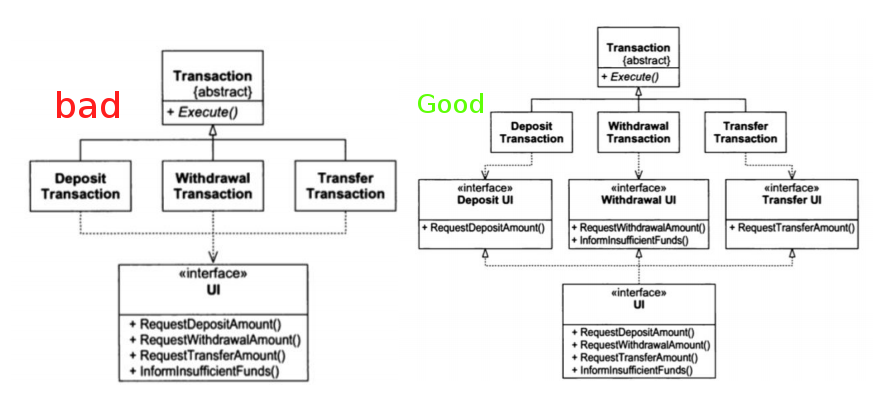
\includegraphics[width=1\textwidth]{topics/bi-wsi-si-09/isp.png}
            \caption{ISP example}
      \end{figure}

      \item \textbf{DIP -- dependency inversion principle}

      \textit{Depend on abstractions, not on concretions.}

      Abstrakce by neměla záviset na detailech. Detaily by měly záviset na abstrakci.
      \begin{figure}[ht]
            \centering
            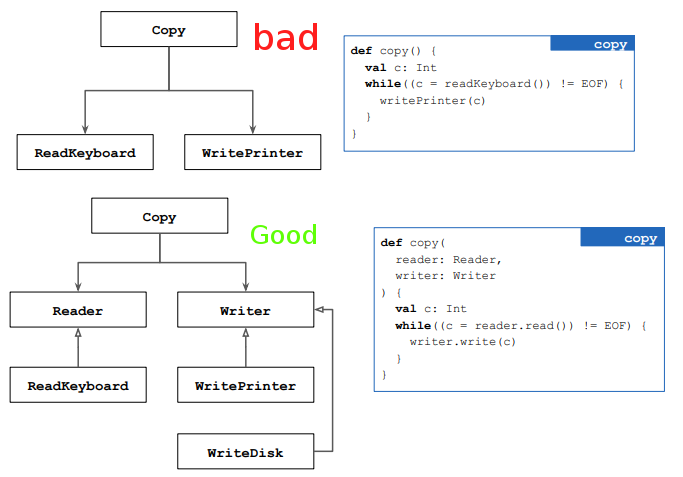
\includegraphics[width=1\textwidth]{topics/bi-wsi-si-09/dip.png}
            \caption{DIP example}
      \end{figure}


\end{itemize}

\section{Závěr k principům OO návrhu}

Malé shrnutí z přednášky o principech OO návrhu:

\begin{itemize}
      % v podstatě slovo od slova přeloženo z velice špatných slidů přednášek BI-OOP
      % konkrétně přednáška 2 slide 64
      \item \textit{podstata je v zasílání zpráv objektům, což vytváří očekávání na polymorfismu},
      \item \textit{volající objekt neví, které konkrétní chování zprávou vyvolá, a ani ho to nezajímá,
      komunikuje s rozhraním volaných objektů, nikoliv s jejich implementací},
      \item provázanost mezi třídami je špatná a vede k \textit{rigid}, \textit{fragile}, \textit{non-reusable} SW,
      \item zamezení vysoké provázanosti lze dosáhnout pomocí dodržování SRP, OCP, LSP, ISP a DIP.
\end{itemize}
%\todo{Toto mi přijde takové moc jednoduše napsané, bylo by možná lepší to popsat trochu formálněji}
\end{document}
